\documentclass[aspectratio=169]{beamer}
\usetheme[theme=blue,logo=logowithtextvi]{HUST} 
\DeclareUnicodeCharacter{221E}{\ensuremath{\infty}}

\usepackage[T5]{fontenc}
\usepackage[utf8]{inputenc}
\usepackage{amsmath}
\usepackage{amsfonts}
\usepackage{amssymb}
\usepackage{graphicx}
\usepackage{adjustbox}
\usepackage{xcolor}
\usepackage{tikz}
\usepackage{minted}
\usepackage{tcolorbox}


\usetikzlibrary{positioning,calc,shapes.symbols,matrix,fit,backgrounds,decorations.pathreplacing,arrows.meta, shapes.geometric}
\definecolor{codeblue}{RGB}{0,90,200}   
\definecolor{codegold}{RGB}{210,160,0}
\definecolor{HUSTBlue}{RGB}{0,51,102}

\setminted{
	breaklines=false,
	autogobble=false,
	obeytabs=true,
	tabsize=2,
	linenos=true,
	showspaces=false,
	space=~,
	baselinestretch=1,
	fontsize=\normalsize,
	rulecolor=\color{black}
}

\newcommand{\placecontent}[4]{%
	\tikz[remember picture,overlay]
	\node[anchor=north west]
	at ([xshift=#1,yshift=-#2]current page.north west)
	{\parbox{#3}{#4}};
}

\graphicspath{{./week 15 resources/}}

\title{\huge CẤU TRÚC DỮ LIỆU VÀ GIẢI THUẬT}
\author{SoICT - HUST}
\date{}

\begin{document}
	
	% 2 slides đầu tiên:
	\HUSTInsertBrandSlide
	\HUSTInsertThemeSlide
	
	% Slide tiêu đề
	{\HUSTUseBackground{onelove.pdf}
		\begin{frame}
			\ifdefstring{\insertaspectratio}{169}{
				\HUSTCornerImage[0.14]{assets/logo/soict_vi_h.pdf}
				\placecontent{0.5cm}{0.33\paperheight}{0.85\paperwidth}{
					\color{\HUSTFrameTitleTextColor}\bfseries\fontsize{22pt}{30pt}\selectfont
					\inserttitle
				}
				\placecontent{0.5cm}{0.50\paperheight}{0.8\paperwidth}{
					\color{\HUSTFrameTitleTextColor}\fontsize{14pt}{14pt}\selectfont
					%Bài học
					\textbf{\large TUẦN 15: ĐỒ THỊ(PHẦN 2)}\\
				}
			}{}
		\end{frame}
	}
	
	% Outline
	\AtBeginSection[]
	{
		\begin{frame}<beamer>
			\frametitle{NỘI DUNG}
			\tableofcontents[currentsection]
		\end{frame}
	}
	
	%Nội dung chính trong slides
	\section{Thuật toán Kruskal và cấu trúc Disjoint Set giải bài toán cây khung nhỏ nhất}
	
	\begin{frame}[t]{THUẬT TOÁN KRUSKAL VÀ CẤU TRÚC DISJOINT SET}
		\small
		\setlength{\leftmargini}{-1.2em}
		
		\begin{itemize}
			\item Bài toán cây khung nhỏ nhất của đồ thị
			\begin{itemize}
				\item Cho đồ thị vô hướng liên thông $G=(V,E)$ trong đó $V=\{1,2,\ldots,n\}$ là tập đỉnh và $E$ là tập cạnh
				\begin{itemize}
					\item $c(u,v)$ là trọng số cạnh $(u,v)$, với mọi $(u,v)\in E$
				\end{itemize}
				
				\item Cây $T=(V,F)$ trong đó $F\subseteq E$ được gọi là một cây khung của $G$
				
				\item Yêu cầu: tìm cây khung của $G$ với trọng số nhỏ nhất
			\end{itemize}
		\end{itemize}
	\end{frame}
	
	\begin{frame}[t]{THUẬT TOÁN KRUSKAL VÀ CẤU TRÚC DISJOINT SET}
		\small
		\setlength{\leftmargini}{-1.2em}
		
		\begin{itemize}
			\item Bài toán cây khung nhỏ nhất của đồ thị
			\begin{itemize}
				\item Cho đồ thị vô hướng liên thông $G=(V,E)$ trong đó $V=\{1,2,\ldots,n\}$ là tập đỉnh và $E$ là tập cạnh
				\begin{itemize}
					\item $c(u,v)$ là trọng số cạnh $(u,v)$, với mọi $(u,v)\in E$
				\end{itemize}
				\item Cây $T=(V,F)$ trong đó $F\subseteq E$ được gọi là một cây khung của $G$
				\item Yêu cầu: tìm cây khung của $G$ với trọng số nhỏ nhất
			\end{itemize}
		\end{itemize}
		
		\vspace{-0.5em}
		
		\begin{columns}[T,onlytextwidth]
			%==================== LEFT: Graph G ====================
			\begin{column}{0.30\textwidth}
				\centering
				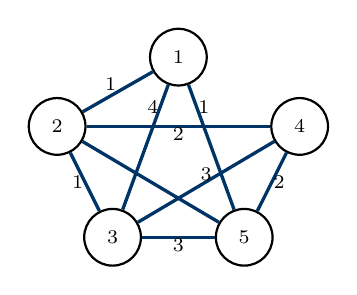
\begin{tikzpicture}[scale=0.88]
					\tikzset{
						v/.style={circle, draw=black, line width=0.8pt, fill=white,
							minimum size=7.2mm, inner sep=0pt, font=\scriptsize},
						e/.style={draw=HUSTBlue, line width=1.2pt},
						w/.style={font=\scriptsize, inner sep=0pt}
					}
					\node[v] (n1) at (0, 1.55) {1};
					\node[v] (n2) at (-1.75, 0.55) {2};
					\node[v] (n4) at ( 1.75, 0.55) {4};
					\node[v] (n3) at (-0.95,-1.05) {3};
					\node[v] (n5) at ( 0.95,-1.05) {5};
					
					% edges (as in hình)
					\draw[e] (n1)--(n2) node[midway, w, above left] {1};
					\draw[e] (n1)--(n3) node[pos=0.18, w, left] {4};
					\draw[e] (n1)--(n5) node[pos=0.18, w, right] {1};
					
					\draw[e] (n2)--(n4) node[midway, w, below] {2};
					\draw[e] (n2)--(n3) node[midway, w, left] {1};
					\draw[e] (n2)--(n5); % (đường chéo có trong hình nhưng không ghi nhãn)
					
					\draw[e] (n3)--(n5) node[midway, w, below] {3};
					\draw[e] (n3)--(n4) node[midway, w, above] {3};
					\draw[e] (n4)--(n5) node[midway, w, right] {2};
				\end{tikzpicture}
				{\footnotesize Đồ thị $G$}
			\end{column}
			
			%==================== ARROW ====================
			\begin{column}{0.10\textwidth}
				\centering
				\vspace{1.7cm}
				{\color{HUSTBlue}\Huge$\Rightarrow$}
			\end{column}
			
			%==================== MIDDLE: Spanning tree T1 ====================
			\begin{column}{0.30\textwidth}
				\centering
				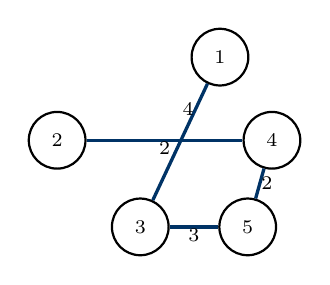
\begin{tikzpicture}[scale=0.88]
					\tikzset{
						v/.style={circle, draw=black, line width=0.8pt, fill=white,
							minimum size=7.2mm, inner sep=0pt, font=\scriptsize},
						e/.style={draw=HUSTBlue, line width=1.2pt},
						w/.style={font=\scriptsize, inner sep=0pt}
					}
					\node[v] (n2) at (-1.55, 0.15) {2};
					\node[v] (n4) at ( 1.55, 0.15) {4};
					\node[v] (n3) at (-0.35,-1.10) {3};
					\node[v] (n5) at ( 1.20,-1.10) {5};
					\node[v] (n1) at ( 0.80, 1.35) {1};
					
					\draw[e] (n2)--(n4) node[midway, w, below] {2};
					\draw[e] (n4)--(n5) node[midway, w, right] {2};
					\draw[e] (n3)--(n5) node[midway, w, below] {3};
					\draw[e] (n3)--(n1) node[pos=0.78, w, left] {4};
				\end{tikzpicture}

				{\footnotesize Cây khung $T_1$, trọng số\\[-0.2em] 11}
			\end{column}
			
			%==================== RIGHT: Spanning tree T2 ====================
			\begin{column}{0.30\textwidth}
				\centering
				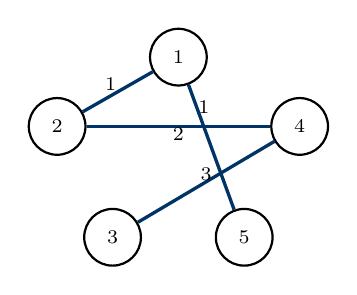
\begin{tikzpicture}[scale=0.88]
					\tikzset{
						v/.style={circle, draw=black, line width=0.8pt, fill=white,
							minimum size=7.2mm, inner sep=0pt, font=\scriptsize},
						e/.style={draw=HUSTBlue, line width=1.2pt},
						w/.style={font=\scriptsize, inner sep=0pt}
					}
					\node[v] (n1) at (0, 1.55) {1};
					\node[v] (n2) at (-1.75, 0.55) {2};
					\node[v] (n4) at ( 1.75, 0.55) {4};
					\node[v] (n3) at (-0.95,-1.05) {3};
					\node[v] (n5) at ( 0.95,-1.05) {5};
					
					\draw[e] (n1)--(n2) node[midway, w, above left] {1};
					\draw[e] (n1)--(n5) node[pos=0.18, w, right] {1};
					\draw[e] (n2)--(n4) node[midway, w, below] {2};
					\draw[e] (n3)--(n4) node[midway, w, above] {3};
				\end{tikzpicture}
				{\footnotesize Cây khung $T_2$, trọng số\\[-0.2em] 7}
			\end{column}
		\end{columns}
	\end{frame}
	
	\begin{frame}[t,fragile]{THUẬT TOÁN KRUSKAL VÀ CẤU TRÚC DISJOINT SET}
		\small
		\setlength{\leftmargini}{-1.2em}
		
		\begin{columns}[T,onlytextwidth]
			% LEFT
			\begin{column}{0.46\textwidth}
				\begin{itemize}
					\item Kruskal là một thuật toán tham lam:
					\begin{itemize}
						\item Ban đầu, lời giải chỉ là tập các đỉnh của $G$
						\item Mỗi bước lặp, ta chọn ra 1 cạnh có trọng số nhỏ nhất để bổ sung vào lời giải với điều kiện không được tạo ra chu trình.
						\item Quá trình lặp sẽ kết thúc khi tất cả các đỉnh của đồ thị được kết nối liên thông với nhau
					\end{itemize}
				\end{itemize}
			\end{column}
			
			% RIGHT
			\hspace*{0.5cm}
			\begin{column}{0.54\textwidth}
				\vspace{-0.2em}
				\begin{tcolorbox}[
					colback=white,
					colframe=HUSTBlue,
					boxrule=0.6pt,
					arc=0pt,
					boxsep=0pt,
					left=-50pt,right=6pt,top=6pt,bottom=6pt,
					height=0.74\textheight,
					valign=top
					]
					\begin{minted}[fontsize=\scriptsize,linenos=false]{text}
						Kruskal(G = (V, E)) {
							T = {};
							L = sort E in a non-decreasing order of weight;
							for (u,v) in L do {
								if T U {(u,v)} does not create a cycle then {
									T = T U {(u,v)};
									if |T| = |V| - 1 then break;
								}
							}
							if |T| < |V| - 1 then
								return NULL;
							else
								return T;
						}
					\end{minted}
				\end{tcolorbox}
			\end{column}
		\end{columns}
	\end{frame}
	
	\begin{frame}[t]{THUẬT TOÁN KRUSKAL VÀ CẤU TRÚC DISJOINT SET}
		\small
		\setlength{\leftmargini}{-1.2em}
		
		\begin{columns}[T,onlytextwidth]
			%==================== LEFT ====================
			\begin{column}{0.58\textwidth}
				\begin{itemize}
					\item Disjoint Set: Là cấu trúc dữ liệu biểu diễn các tập không giao nhau với 2 thao tác chính
					\begin{itemize}
						\item Find(x): trả về định danh của tập chứa x
						\item Unify(r1, r2): Hợp nhất 2 tập hợp định danh là r1 và r2 làm một
					\end{itemize}
				\end{itemize}
			\end{column}
			
			%==================== RIGHT ====================
			\begin{column}{0.42\textwidth}
				\centering
				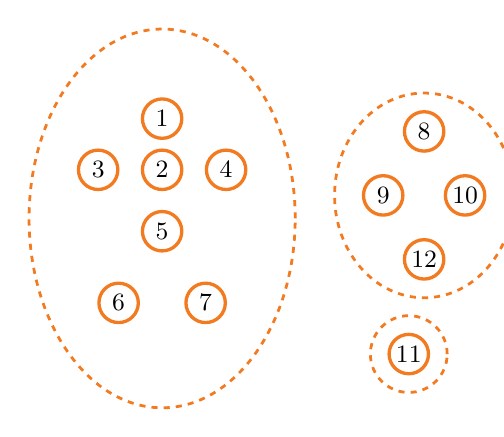
\begin{tikzpicture}[x=0.65cm,y=0.65cm]
					\definecolor{dsorange}{RGB}{242,122,33}
					\tikzset{
						elem/.style={
							circle,
							draw=dsorange,
							line width=1.2pt,
							minimum size=5mm,
							inner sep=0pt,
							font=\small
						},
						setbd/.style={
							draw=dsorange,
							line width=1.0pt,
							dashed,
							dash pattern=on 2.2pt off 2.2pt
						}
					}
					
					% ======= Oval trái (tập {1..7}) =======
					\draw[setbd] (0.0,0.6) ellipse [x radius=2.6, y radius=3.7];
					
					\node[elem] at ( 0.0, 2.55) {1};
					\node[elem] at (-1.25,1.55) {3};
					\node[elem] at ( 0.0, 1.55) {2};
					\node[elem] at ( 1.25,1.55) {4};
					\node[elem] at ( 0.0, 0.35) {5};
					\node[elem] at (-0.85,-1.05) {6};
					\node[elem] at ( 0.85,-1.05) {7};
					
					\hspace*{0.5cm}
					
					% ======= Oval phải (tập {8,9,10,12}) =======
					\draw[setbd] (4.35,1.05) ellipse [x radius=1.75, y radius=2.00];
					
					\node[elem] at (4.35,2.30) {8};
					\node[elem] at (3.55,1.05) {9};
					\node[elem] at (5.15,1.05) {10};
					\node[elem] at (4.35,-0.20) {12};
					
					% ======= Tập riêng {11} (dưới, hơi lệch trái) =======
					\draw[setbd] (4.05,-2.05) circle [radius=0.75];
					\node[elem] at (4.05,-2.05) {11};
				\end{tikzpicture}
			\end{column}
		\end{columns}
	\end{frame}
	
	\begin{frame}[t]{THUẬT TOÁN KRUSKAL VÀ CẤU TRÚC DISJOINT SET}
		\small
		\setlength{\leftmargini}{-1.2em}
		
		\begin{columns}[T,onlytextwidth]
			%==================== LEFT ====================
			\begin{column}{0.45\textwidth}
				\begin{itemize}
					\item Disjoint Set: Là cấu trúc dữ liệu biểu diễn các tập không giao nhau với 2 thao tác chính
					\begin{itemize}
						\item Find(x): trả về định danh của tập chứa x
						\item Unify(u, v): Hợp nhất 2 tập hợp định danh là u và v làm một
					\end{itemize}
				\end{itemize}
			\end{column}
			
			%==================== RIGHT ====================
			\begin{column}{0.55\textwidth}
				\centering
				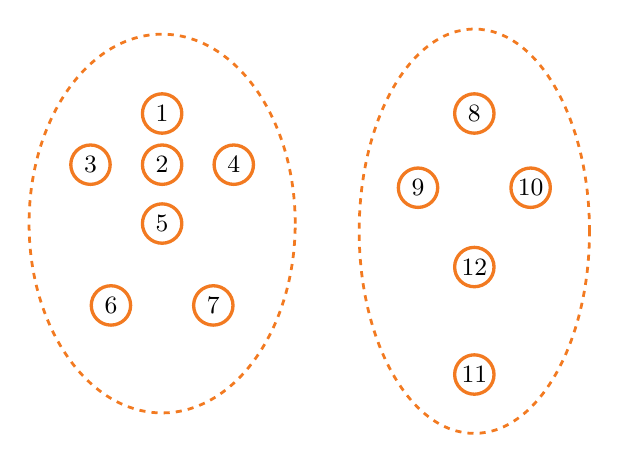
\begin{tikzpicture}[x=0.65cm,y=0.65cm]
					\definecolor{dsorange}{RGB}{242,122,33}
					\tikzset{
						elem/.style={
							circle,
							draw=dsorange,
							line width=1.2pt,
							minimum size=5mm,
							inner sep=0pt,
							font=\small
						},
						setbd/.style={
							draw=dsorange,
							line width=1.0pt,
							dashed,
							dash pattern=on 2.2pt off 2.2pt
						}
					}
					
					% ======= Oval trái: {1..7} =======
					\draw[setbd] (0.0,0.85) ellipse [x radius=2.6, y radius=3.7];
					
					\node[elem] at ( 0.0, 3.00) {1};
					\node[elem] at (-1.40,2.00) {3};
					\node[elem] at ( 0.0, 2.00) {2};
					\node[elem] at ( 1.40,2.00) {4};
					\node[elem] at ( 0.0, 0.85) {5};
					\node[elem] at (-1.00,-0.75) {6};
					\node[elem] at ( 1.00,-0.75) {7};
					
					% ======= Oval phải: {8,9,10,12,11} =======
					\draw[setbd] (6.10,0.70) ellipse [x radius=2.25, y radius=3.95];
					
					\node[elem] at (6.10, 3.00) {8};
					\node[elem] at (5.00, 1.55) {9};
					\node[elem] at (7.20, 1.55) {10};
					\node[elem] at (6.10, 0.00) {12};
					\node[elem] at (6.10,-2.10) {11};
				\end{tikzpicture}
			\end{column}
		\end{columns}
	\end{frame}
	
	\begin{frame}[t]{THUẬT TOÁN KRUSKAL VÀ CẤU TRÚC DISJOINT SET}
		\small
		\setlength{\leftmargini}{-1.2em}
		
		\begin{columns}[T,onlytextwidth]
			%==================== LEFT: nội dung ====================
			\begin{column}{0.45\textwidth}
				\begin{itemize}
					\item Disjoint Set: Là cấu trúc dữ liệu biểu diễn các tập không giao nhau với 2 thao tác chính
					\begin{itemize}
						\item Find(x): trả về định danh của tập chứa x
						\item Unify(u, v): Hợp nhất 2 tập hợp định danh là u và v làm một
					\end{itemize}
					
					\item Mỗi tập được biểu diễn bởi cây có gốc
					\begin{itemize}
						\item Mỗi nút của cây là một phần tử
						\item Mỗi nút $x$ có 1 nút cha duy nhất $p[x]$ (cha của nút gốc là chính nó)
						\item Nút gốc là định danh của tập
					\end{itemize}
				\end{itemize}
			\end{column}
			
			%==================== RIGHT: hình minh hoạ ====================
			\begin{column}{0.55\textwidth}
				\centering
				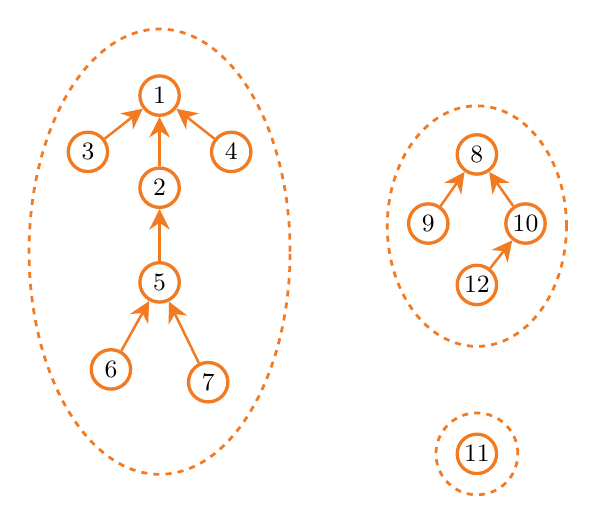
\begin{tikzpicture}[x=0.65cm,y=0.65cm]
					\definecolor{dsorange}{RGB}{242,122,33}
					\tikzset{
						elem/.style={
							circle, draw=dsorange, line width=1.2pt,
							minimum size=5mm, inner sep=0pt, font=\small
						},
						setbd/.style={
							draw=dsorange, line width=1.0pt,
							dashed, dash pattern=on 2.2pt off 2.2pt
						},
						par/.style={
							-{Stealth[length=2.6mm,width=2.6mm]},
							draw=dsorange, line width=0.9pt
						}
					}
					
					% ======= Tập {1..7}: cây có gốc 1 =======
					\draw[setbd] (0.0,1.05) ellipse [x radius=2.55, y radius=4.35];
					
					\node[elem] (a1) at ( 0.00, 4.10) {1};
					\node[elem] (a3) at (-1.40, 3.00) {3};
					\node[elem] (a2) at ( 0.00, 2.30) {2};
					\node[elem] (a4) at ( 1.40, 3.00) {4};
					\node[elem] (a5) at ( 0.00, 0.45) {5};
					\node[elem] (a6) at (-0.95,-1.25) {6};
					\node[elem] (a7) at ( 0.95,-1.5) {7};
					
					\draw[par] (a3) -- (a1);
					\draw[par] (a2) -- (a1);
					\draw[par] (a4) -- (a1);
					\draw[par] (a5) -- (a2);
					\draw[par] (a6) -- (a5);
					\draw[par] (a7) -- (a5);
					
					% ======= Tập {8,9,10,12}: cây có gốc 8 =======
					\draw[setbd] (6.20,1.55) ellipse [x radius=1.75, y radius=2.35];
					
					\node[elem] (b8)  at (6.20, 2.95) {8};
					\node[elem] (b9)  at (5.25, 1.60) {9};
					\node[elem] (b10) at (7.15, 1.60) {10};
					\node[elem] (b12) at (6.20, 0.40) {12};
					
					\draw[par] (b9)  -- (b8);
					\draw[par] (b10) -- (b8);
					\draw[par] (b12) -- (b10);
					
					% ======= Tập {11}: một nút riêng =======
					\draw[setbd] (6.20,-2.90) circle [radius=0.80];
					\node[elem] (c11) at (6.20,-2.90) {11};
					
				\end{tikzpicture}
			\end{column}
		\end{columns}
	\end{frame}
	
	\begin{frame}[t,fragile]{THUẬT TOÁN KRUSKAL VÀ CẤU TRÚC DISJOINT SET}
		\small
		\setlength{\leftmargini}{-1.2em}
		
		\begin{columns}[T,onlytextwidth]
			%==================== LEFT ====================
			\begin{column}{0.55\textwidth}
				\begin{itemize}
					\item Thao tác Find(x):
					\begin{itemize}
						\item Xuất phát từ $x$, liên tiếp truy cập đến nút cha để tìm đến nút gốc
						\item Độ phức tạp tỉ lệ với độ dài của đường đi từ $x$ đến gốc
						\item Path Compression: trong quá trình đi từ $x$ đến gốc, các nút trên đường đi sẽ được gán như là nút con trực tiếp của nút gốc để giảm độ dài đường đi từ các nút này đến gốc trong các bước lặp sau
					\end{itemize}
				\end{itemize}

				
				\begin{tcolorbox}[
					colback=white,
					colframe=HUSTBlue,
					boxrule=0.6pt,
					arc=0pt,
					left=-40pt,right=8pt,top=6pt,bottom=6pt
					]
					\begin{minted}[fontsize=\footnotesize,linenos=false]{c}
						Find(x){
							if(x != p[x]) p[x] = Find(p[x]);
							return p[x];
						}
					\end{minted}
				\end{tcolorbox}
			\end{column}
			
			%==================== RIGHT ====================
			\begin{column}{0.45\textwidth}
				\centering
				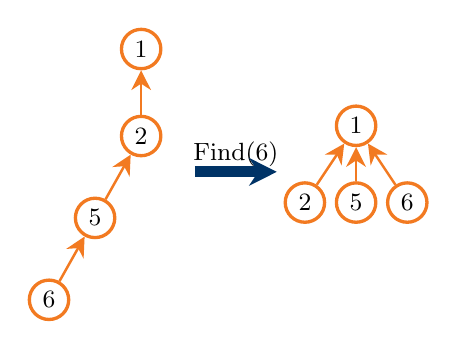
\begin{tikzpicture}[x=0.65cm,y=0.65cm]
					\definecolor{dsorange}{RGB}{242,122,33}
					\tikzset{
						elem/.style={circle, draw=dsorange, line width=1.2pt,
							minimum size=5mm, inner sep=0pt, font=\small},
						par/.style={-{Stealth[length=2.5mm,width=2.5mm]},
							draw=dsorange, line width=0.9pt},
						arrowB/.style={-{Stealth[length=3.5mm,width=3.5mm]},
							draw=HUSTBlue, line width=4pt}
					}
					
					% BEFORE
					\node[elem] (n1) at (0.0, 2.4) {1};
					\node[elem] (n2) at (0.0, 0.7) {2};
					\node[elem] (n5) at (-0.9, -0.9) {5};
					\node[elem] (n6) at (-1.8,-2.5) {6};
					
					\draw[par] (n2) -- (n1);
					\draw[par] (n5) -- (n2);
					\draw[par] (n6) -- (n5);
					
					\node[font=\small] at (1.85,0.35) {Find(6)};
					\draw[arrowB] (1.05,0.0) -- (2.65,0.0);
					
					% AFTER
					\node[elem] (r1) at (4.2, 0.9) {1};
					\node[elem] (r2) at (3.2,-0.6) {2};
					\node[elem] (r5) at (4.2,-0.6) {5};
					\node[elem] (r6) at (5.2,-0.6) {6};
					
					\draw[par] (r2) -- (r1);
					\draw[par] (r5) -- (r1);
					\draw[par] (r6) -- (r1);
				\end{tikzpicture}
			\end{column}
		\end{columns}
	\end{frame}
	
	\begin{frame}[t,fragile]{THUẬT TOÁN KRUSKAL VÀ CẤU TRÚC DISJOINT SET}
		\small
		\setlength{\leftmargini}{-1.2em}
		
		\begin{columns}[T,onlytextwidth]
			%==================== LEFT: bullet + code ====================
			\begin{column}{0.45\textwidth}
				\begin{itemize}
					\item Thao tác Unify($u,v$):
					\begin{itemize}
						\item Cho $u$ là con của $v$ hoặc $v$ là con của $u$ tuỳ thuộc độ cao của nút nào nhỏ hơn
						\item Mỗi nút, duy trì $r[x]$ thể hiện độ cao của nút $x$
					\end{itemize}
				\end{itemize}
				
				\vspace{0.5em}
				
				\begin{tcolorbox}[
					colback=white,
					colframe=HUSTBlue,
					boxrule=0.6pt,
					arc=0pt,
					left=-50pt,right=8pt,top=6pt,bottom=6pt
					]
					\begin{minted}[fontsize=\scriptsize,linenos=false]{text}
						Unify(x, y){
							if(r[x] > r[y]) p[y] = x;
							else{
								p[x] = y;
								if(r[x] == r[y]) r[y] = r[y] + 1;
							}
						}
					\end{minted}
				\end{tcolorbox}
			\end{column}
			
			%==================== RIGHT: 그림 DSU + mũi tên 8 -> 1 ====================
			\begin{column}{0.55\textwidth}
				\centering
				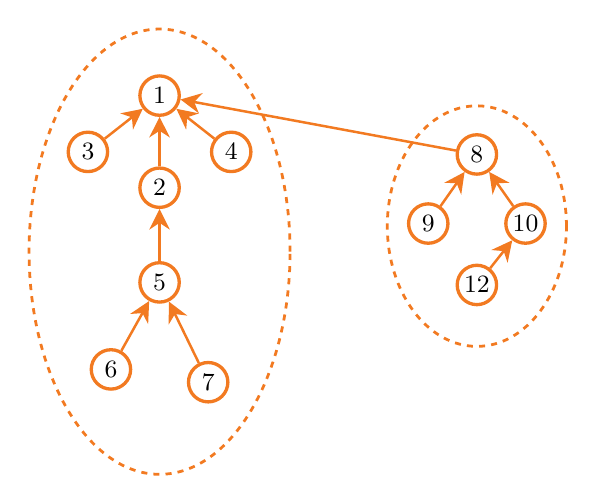
\begin{tikzpicture}[x=0.65cm,y=0.65cm]
					\definecolor{dsorange}{RGB}{242,122,33}
					\tikzset{
						elem/.style={
							circle, draw=dsorange, line width=1.2pt,
							minimum size=5mm, inner sep=0pt, font=\small
						},
						setbd/.style={
							draw=dsorange, line width=1.0pt,
							dashed, dash pattern=on 2.2pt off 2.2pt
						},
						par/.style={
							-{Stealth[length=2.6mm,width=2.6mm]},
							draw=dsorange, line width=0.9pt
						}
					}
					
					% ======= Tập {1..7}: cây có gốc 1 =======
					\draw[setbd] (0.0,1.05) ellipse [x radius=2.55, y radius=4.35];
					
					\node[elem] (a1) at ( 0.00, 4.10) {1};
					\node[elem] (a3) at (-1.40, 3.00) {3};
					\node[elem] (a2) at ( 0.00, 2.30) {2};
					\node[elem] (a4) at ( 1.40, 3.00) {4};
					\node[elem] (a5) at ( 0.00, 0.45) {5};
					\node[elem] (a6) at (-0.95,-1.25) {6};
					\node[elem] (a7) at ( 0.95,-1.50) {7};
					
					\draw[par] (a3) -- (a1);
					\draw[par] (a2) -- (a1);
					\draw[par] (a4) -- (a1);
					\draw[par] (a5) -- (a2);
					\draw[par] (a6) -- (a5);
					\draw[par] (a7) -- (a5);
					
					% ======= Tập {8,9,10,12}: cây có gốc 8 =======
					\draw[setbd] (6.20,1.55) ellipse [x radius=1.75, y radius=2.35];
					
					\node[elem] (b8)  at (6.20, 2.95) {8};
					\node[elem] (b9)  at (5.25, 1.60) {9};
					\node[elem] (b10) at (7.15, 1.60) {10};
					\node[elem] (b12) at (6.20, 0.40) {12};
					
					\draw[par] (b9)  -- (b8);
					\draw[par] (b10) -- (b8);
					\draw[par] (b12) -- (b10);
					
					% ======= Mũi tên minh hoạ Unify: 8 -> 1 =======
					\draw[par] (b8) -- (a1);
					
				\end{tikzpicture}
			\end{column}
		\end{columns}
	\end{frame}
	
	\begin{frame}[t,fragile]{THUẬT TOÁN KRUSKAL VÀ CẤU TRÚC DISJOINT SET}
		\vspace{-0.5cm}
		\begin{columns}[T,onlytextwidth]
			%==================== LEFT BOX ====================
			\begin{column}{0.45\textwidth}
				\begin{tcolorbox}[
					colback=white,
					colframe=HUSTBlue,
					boxrule=0.6pt,
					arc=0pt,
					left=-40pt,right=10pt,top=8pt,bottom=8pt
					]
					\begin{minted}[fontsize=\scriptsize,linenos=false]{text}
						makeSet(x){
							p[x] = x; r[x] = 0;
						}
						
						Find(x){
							if(x != p[x]) p[x] = Find(p[x]);
							return p[x];
						}
						
						Unify(x, y){
							if(r[x] > r[y]) p[y] = x;
							else{
								p[x] = y;
								if(r[x] == r[y]) r[y] = r[y] + 1;
							}
						}
					\end{minted}
				\end{tcolorbox}
			\end{column}
			
			\hspace*{0.5cm}
			%==================== RIGHT BOX ====================
			\begin{column}{0.55\textwidth}
				\begin{tcolorbox}[
					colback=white,
					colframe=HUSTBlue,
					boxrule=0.6pt,
					arc=0pt,
					left=-50pt,right=10pt,top=8pt,bottom=8pt
					]
					\begin{minted}[fontsize=\scriptsize,linenos=false]{text}
						KruskalWithDisjointSet(G = (V, E)){
							T = {};
							for v in V do makeSet(v);
							L = sort E in a non-decreasing order of weight;
							for (u,v) in L do {
								ru = Find(u);
								rv = Find(v);
								if ru != rv then {
									Unify(ru, rv);
									T = T U {(u,v)};
									if |T| == |V| - 1 then break;
								}
							}							
							if |T| < |V| - 1 then return {};
							return T;
						}
					\end{minted}
				\end{tcolorbox}
			\end{column}
		\end{columns}
	\end{frame}
	
	%==================== SLIDE: Minh hoạ dữ liệu vào/ra ====================
	\begin{frame}[t]{THUẬT TOÁN KRUSKAL VÀ CẤU TRÚC DISJOINT SET}
		\small
		\setlength{\leftmargini}{-1.2em}
		
		\begin{columns}[T,onlytextwidth]
			%==================== LEFT: bullet ====================
			\begin{column}{0.62\textwidth}
				\begin{itemize}
					\item Minh hoạ với ngôn ngữ C
					
					\item Dữ liệu
					\begin{itemize}
						\item Dòng 1: ghi 2 số nguyên dương $n$ và $m$ tương ứng là số đỉnh và số cạnh của $G$
						\ \ $(1 \le n, m \le 10^5)$
						
						\item Dòng $i$ $(i=1,2,\ldots,m)$: ghi 3 số nguyên dương $u$, $v$ and $c$ trong đó $c$ là trọng số cạnh $(u,v)$
					\end{itemize}
					
					\item Kết quả
					\begin{itemize}
						\item Ghi ra trọng số của cây khung nhỏ nhất tìm được
					\end{itemize}
				\end{itemize}
			\end{column}
			
			%==================== RIGHT: I/O table ====================
			\begin{column}{0.38\textwidth}
				\centering
				\vspace{0.9cm} % chỉnh lên/xuống để khớp đúng vị trí như slide mẫu
				
				\renewcommand{\arraystretch}{1.15}
				\setlength{\tabcolsep}{8pt}
				
				\begin{tabular}{|p{0.55\linewidth}|p{0.33\linewidth}|}
					\hline
					\textbf{stdin} & \textbf{stdout} \\
					\hline
					\begin{minipage}[t]{\linewidth}\raggedright\footnotesize
						5 8\\
						1 2 1\\
						1 3 4\\
						1 5 1\\
						2 4 2\\
						2 5 1\\
						3 4 3\\
						3 5 3\\
						4 5 2
					\end{minipage}
					&
					\begin{minipage}[t]{\linewidth}\raggedright\footnotesize
						7
					\end{minipage}
					\\
					\hline
				\end{tabular}
			\end{column}
		\end{columns}
	\end{frame}
	
	%==================== SLIDE: Code (khai báo + DSU) ====================
	\begin{frame}[t,fragile]{THUẬT TOÁN KRUSKAL VÀ CẤU TRÚC DISJOINT SET}
		\vspace{-0.5cm}
		\setlength{\leftmargini}{-1.2em}
		
		\begin{columns}[T,onlytextwidth]
			%==================== LEFT BOX ====================
			\begin{column}{0.49\textwidth}
				\begin{tcolorbox}[
					colback=white,
					colframe=HUSTBlue,
					boxrule=0.6pt,
					arc=0pt,
					left=-40pt,right=8pt,top=8pt,bottom=8pt
					]
					\begin{minted}[fontsize=\scriptsize,linenos=false]{text}
						#include <stdio.h>
						#define MAX 100001
						
						// data structure for input graph
						int N, M;
						
						int u[MAX];
						int v[MAX];
						int c[MAX];
						int ET[MAX];
						int nET;
						
						// data structure for disjoint-set
						int r[MAX]; // r[v] is rank of set v
						int p[MAX]; // p[v] is parent of v
						long long rs;
					\end{minted}
				\end{tcolorbox}
			\end{column}
			
			%==================== RIGHT BOX ====================
			\begin{column}{0.49\textwidth}
				\begin{tcolorbox}[
					colback=white,
					colframe=HUSTBlue,
					boxrule=0.6pt,
					arc=0pt,
					left=-40pt,right=8pt,top=8pt,bottom=8pt
					]
					\begin{minted}[fontsize=\scriptsize,linenos=false]{text}
						void unify(int x, int y){
							if(r[x] > r[y]) p[y] = x;
							else{
								p[x] = y;
								if(r[x] == r[y]) r[y] = r[y] + 1;
							}
						}
						
						void makeSet(int x){
							p[x] = x;   r[x] = 0;
						}
						
						int findSet(int x){
							if(x != p[x]) p[x] = findSet(p[x]);
							return p[x];
						}
					\end{minted}
				\end{tcolorbox}
			\end{column}
		\end{columns}
	\end{frame}
	
	%==================== SLIDE: Code (sort cạnh bằng QuickSort) ====================
	\begin{frame}[t,fragile]{THUẬT TOÁN KRUSKAL VÀ CẤU TRÚC DISJOINT SET}
		\vspace{-0.5cm}
		\setlength{\leftmargini}{-1.2em}
		
		\begin{columns}[T,onlytextwidth]
			%==================== LEFT BOX ====================
			\begin{column}{0.49\textwidth}
				\begin{tcolorbox}[
					colback=white,
					colframe=HUSTBlue,
					boxrule=0.6pt,
					arc=0pt,
					left=-53pt,right=8pt,top=8pt,bottom=8pt
					]
					\begin{minted}[fontsize=\scriptsize,linenos=false]{text}
						void swapEdge(int i, int j){
							int tmp = c[i]; c[i] = c[j]; c[j] = tmp;
							tmp = u[i]; u[i] = u[j]; u[j] = tmp;
							tmp = v[i]; v[i] = v[j]; v[j] = tmp;
						}
						
						int partition(int L, int R, int index){
							int pivot = c[index]; swapEdge(index, R);
							int storeIndex = L;
							
							for(int i = L; i <= R-1; i++){
								if(c[i] < pivot){
									swapEdge(storeIndex, i); storeIndex++;
								}
							}
							swapEdge(storeIndex, R); return storeIndex;
						}
					\end{minted}
				\end{tcolorbox}
			\end{column}
			
			%==================== RIGHT BOX ====================
			\begin{column}{0.49\textwidth}
				\begin{tcolorbox}[
					colback=white,
					colframe=HUSTBlue,
					boxrule=0.6pt,
					arc=0pt,
					left=-40pt,right=8pt,top=8pt,bottom=8pt
					]
					\begin{minted}[fontsize=\scriptsize,linenos=false]{text}
						void quickSort(int L, int R){
							if(L < R){
								int index = (L+R)/2;
								
								index = partition(L, R, index);
								
								if(L < index) quickSort(L, index-1);
								
								if(index < R) quickSort(index+1, R);
							}
						}
						
						void sort(){
							quickSort(0, M-1);
						}
					\end{minted}
				\end{tcolorbox}
			\end{column}
		\end{columns}
	\end{frame}
	
	%==================== SLIDE: Code (kruskal + input/main) ====================
	\begin{frame}[t,fragile]{THUẬT TOÁN KRUSKAL VÀ CẤU TRÚC DISJOINT SET}
		\vspace{-0.5cm}
		\setlength{\leftmargini}{-1.2em}
		
		\begin{columns}[T,onlytextwidth]
			%==================== LEFT BOX ====================
			\begin{column}{0.49\textwidth}
				\begin{tcolorbox}[
					colback=white,
					colframe=HUSTBlue,
					boxrule=0.6pt,
					arc=0pt,
					left=-40pt,right=8pt,top=8pt,bottom=8pt
					]
					\begin{minted}[fontsize=\scriptsize,linenos=false]{text}
						void kruskal(){
							for(int x = 1; x <= N; x++) makeSet(x);
							sort(); rs = 0; int nET = 0;
							
							for(int i = 0; i < M; i++){
								int ru = findSet(u[i]);
								int rv = findSet(v[i]);
								
								if(ru != rv){
									unify(ru, rv);
									nET++; rs += c[i];
									if(nET == N-1) break;
								}
							}
							
							printf("%lld", rs);
						}
					\end{minted}
				\end{tcolorbox}
			\end{column}
			
			%==================== RIGHT BOX ====================
			\begin{column}{0.49\textwidth}
				\begin{tcolorbox}[
					colback=white,
					colframe=HUSTBlue,
					boxrule=0.6pt,
					arc=0pt,
					left=-40pt,right=8pt,top=8pt,bottom=8pt
					]
					\begin{minted}[fontsize=\scriptsize,linenos=false]{text}
						void input(){
							scanf("%d%d", &N, &M);
							
							for(int i = 0; i < M; i++){
								scanf("%d%d%d", &u[i], &v[i], &c[i]);
							}
						}
						
						int main(){
							input();
							kruskal();
						}
					\end{minted}
				\end{tcolorbox}
			\end{column}
		\end{columns}
	\end{frame}
	
	
	\section{Thuật toán Dijkstra và cấu trúc Priority Queue giải bài toán đường đi ngắn nhất}
	
	%==================== SLIDE: Dijkstra - bài toán đường đi ngắn nhất ====================
	\begin{frame}[t]{THUẬT TOÁN DIJKSTRA VÀ CẤU TRÚC PRIORITY QUEUE}
		\small
		\setlength{\leftmargini}{-1.2em}
		
		\begin{itemize}
			\item Bài toán đường đi ngắn nhất giữa 2 đỉnh trên đồ thị trọng số không âm
			\begin{itemize}
				\item Cho đồ thị có hướng liên thông $G=(V,E)$ trong đó $V=\{1,2,\ldots,n\}$ là tập đỉnh và $E$ là tập cung
				\begin{itemize}
					\item $c(u,v)$ là trọng số không âm của cung $(u,v)$, với mọi $(u,v)\in E$
				\end{itemize}
				\item Yêu cầu: Cho 2 đỉnh $s$ và $t$ thuộc $G$, hãy tìm đường đi có tổng trọng số nhỏ nhất trên $G$
			\end{itemize}
		\end{itemize}
		\vspace*{-0.3cm}
		
		\begin{center}
			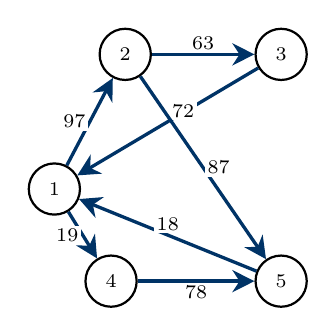
\begin{tikzpicture}[x=0.9cm,y=0.9cm]
				\tikzset{
					v/.style={circle, draw=black, line width=0.8pt, fill=white,
						minimum size=6.5mm, inner sep=0pt, font=\scriptsize},
					e/.style={-{Stealth[length=2.8mm,width=2.8mm]}, draw=HUSTBlue, line width=1.2pt},
					w/.style={font=\scriptsize, inner sep=1pt, fill=white}
				}
				
				% ======= Nodes (bố cục giống hình) =======
				\node[v] (n2) at (0.0,  1.9) {2};
				\node[v] (n3) at (2.2,  1.9) {3};
				\node[v] (n1) at (-1.0, 0.0) {1};
				\node[v] (n4) at (-0.2,-1.3) {4};
				\node[v] (n5) at ( 2.2,-1.3) {5};
				
				% ======= Directed weighted edges =======
				\draw[e] (n1) -- (n2) node[midway, w, left] {97};
				\draw[e] (n2) -- (n3) node[midway, w, above] {63};
				\draw[e] (n3) -- (n1) node[midway, w, above right] {72};
				\draw[e] (n2) -- (n5) node[midway, w, right] {87};
				\draw[e] (n5) -- (n1) node[midway, w, above] {18};
				\draw[e] (n1) -- (n4) node[midway, w, left] {19};
				\draw[e] (n4) -- (n5) node[midway, w, below] {78};
			\end{tikzpicture}
			
			
			{\normalsize
				Đồ thị $G$: đường đi ngắn nhất từ 1 đến 5 là $1-4-5$ với độ dài bằng $19 + 78 = 97$
			}
		\end{center}
	\end{frame}
	
	\begin{frame}[t]{THUẬT TOÁN DIJKSTRA VÀ CẤU TRÚC PRIORITY QUEUE}
		\small
		\setlength{\leftmargini}{-1.2em}
		
		\begin{itemize}
			\item Cấu trúc dữ liệu biểu diễn đồ thị $G$ sử dụng danh sách kề
			\begin{itemize}
				\item $A[u]$ là tập các cung $e$ đi ra khỏi đỉnh $u$, mọi $u \in V$.
				\item Với mỗi cung $e$ đi ra khỏi đỉnh $u$ thì $e.id$ là đỉnh còn lại của $e$ và $e.w$ là trọng số cung
				\begin{itemize}
					\item Ví dụ: cung $e=(u,v)$ là một cung đi ra khỏi $u$ có trọng số 10, khi đó $e.id=v$ và $e.w=10$
				\end{itemize}
			\end{itemize}
		\end{itemize}
	\end{frame}
	
	%==================== SLIDE: Dijkstra + Pseudocode ====================
	\begin{frame}[t,fragile]{THUẬT TOÁN DIJKSTRA VÀ CẤU TRÚC PRIORITY QUEUE}
		\small
		\setlength{\leftmargini}{-1.2em}
		
		\begin{columns}[T,onlytextwidth]
			% LEFT: mô tả
			\begin{column}{0.46\textwidth}
				\begin{itemize}
					\item Thuật toán Dijkstra
					\begin{itemize}
						\item Với mỗi đỉnh $v$ của $G$, ta duy trì một đường đi cận trên $P[v]$ của đường đi ngắn nhất từ $s$ đến $v$.
						Ký hiệu $d[v]$ là độ dài của $P[v]$. Đường đi cận trên này sẽ được làm tốt dần lên (độ dài giảm dần) qua các bước lặp.
						
						\item Nếu tồn tại một đỉnh $u$ sao cho $d[v] > d[u] + c(u,v)$ thì ta làm tốt đường đi cận trên $P[v]$ bằng đường đi $P[u]$ nối thêm cung $(u,v)$,
						đồng thời cập nhật $d[v] = d[u] + c(u,v)$.
					\end{itemize}
				\end{itemize}
			\end{column}
			
			% RIGHT: giả mã (minted)
			\begin{column}{0.50\textwidth}
				\vspace{-0.2em}
				\begin{tcolorbox}[
					colback=white,
					colframe=HUSTBlue,
					boxrule=0.6pt,
					arc=0pt,
					boxsep=0pt,
					left=-50pt,right=8pt,top=6pt,bottom=6pt,
					]
					\begin{minted}[fontsize=\scriptsize,linenos=false]{text}
						Dijkstra(G = (V, E)){
							for v in V do d[v] = ∞;
							
							d[s] = 0;  F = V;
							
							while F not empty do {
								u = select u from F s.t. d[u] is minimal;
								if u = t then break;
								
								F = F \ {u};
								
								for e in A[u] do {
									if d[e.id] > d[u] + e.w then
									d[e.id] = d[u] + e.w;
								}
							}
							
							return d[t];
						}
					\end{minted}
				\end{tcolorbox}
			\end{column}
		\end{columns}
	\end{frame}
	
	%==================== SLIDE: Priority Queue (min-heap) ====================
	\begin{frame}[t]{THUẬT TOÁN DIJKSTRA VÀ CẤU TRÚC PRIORITY QUEUE}
		\small
		\setlength{\leftmargini}{-1.2em}
		
		\begin{columns}[T,onlytextwidth]
			%==================== LEFT: bullet ====================
			\begin{column}{0.45\textwidth}
				\begin{itemize}
					\item Priority Queue (hàng đợi ưu tiên)
					\begin{itemize}
						\item Cấu trúc dữ liệu lưu trữ các cặp phần tử $v$ và khóa của nó $d[v]$, với 2 thao tác chính:
						\begin{itemize}
							\item push($v$, $d[v]$): đưa cặp $(v, d[v])$ vào hàng đợi ưu tiên\\
							hoặc cập nhật lại khóa của $v$ nếu phần tử (cặp) định\\
							danh $v$ đã tồn tại
							\item deleteMin(): loại bỏ cặp $(v, d[v])$ có khóa $d[v]$ nhỏ\\
							nhất trong số các cặp trong hàng đợi ưu tiên và trả\\
							về phần tử $v$.
						\end{itemize}
					\end{itemize}
				\end{itemize}
			\end{column}
			
			%==================== RIGHT: heap picture ====================
			\begin{column}{0.50\textwidth}
				\centering
				\vspace{1.05cm}
				
				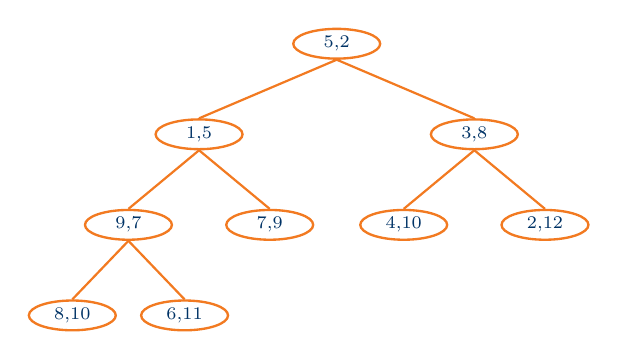
\begin{tikzpicture}[scale=0.92, transform shape,
					grow=down,
					level 1/.style={level distance=1.25cm, sibling distance=3.80cm},
					level 2/.style={level distance=1.25cm, sibling distance=1.95cm},
					level 3/.style={level distance=1.25cm, sibling distance=1.55cm}
					]
					\definecolor{pqorange}{RGB}{242,122,33}
					\tikzset{
						pqnode/.style={
							shape=ellipse,
							draw=pqorange,
							line width=0.85pt,
							fill=white,
							minimum width=12mm,
							minimum height=.0mm,
							inner sep=1.2pt,
							font=\scriptsize,
							text=HUSTBlue
						},
						pqedge/.style={draw=pqorange,line width=0.8pt},
						edge from parent/.style={pqedge},
						edge from parent path={(\tikzparentnode.south) -- (\tikzchildnode.north)}
					}
					
					% Cây đúng như hình: (5,2) -> (1,5),(3,8) ...
					\node[pqnode]{5,2}
					child { node[pqnode]{1,5}
						child { node[pqnode]{9,7}
							child { node[pqnode]{8,10} }
							child { node[pqnode]{6,11} }
						}
						child { node[pqnode]{7,9} }
					}
					child { node[pqnode]{3,8}
						child { node[pqnode]{4,10} }
						child { node[pqnode]{2,12} }
					};
				\end{tikzpicture}
			\end{column}
		\end{columns}
	\end{frame}
	
	%==================== SLIDE: Priority Queue - Cài đặt bằng mảng (Min-Heap) ====================
	\begin{frame}[t]{THUẬT TOÁN DIJKSTRA VÀ CẤU TRÚC PRIORITY QUEUE}
		\small
		\setlength{\leftmargini}{-1.2em}
		
		\begin{columns}[T,onlytextwidth]
			%==================== LEFT: bullet (GIẢM NESTING) ====================
			\begin{column}{0.50\textwidth}
				\begin{itemize}
					\item Priority Queue (hàng đợi ưu tiên)
					\begin{itemize}
						\item Cài đặt:
						\begin{itemize}
							\item Sử dụng mảng với các phần tử được đánh số $0,1,2,\ldots$;
							mỗi phần tử lưu cặp $(v, d[v])$ với $v$ là định danh và $d[v]$ là khóa.
							
							\item Mảng được nhìn dưới góc độ một cây nhị phân đầy đủ:
							phần tử có số thứ tự $i$ thì con trái có số thứ tự $2i+1$ và con phải có số thứ tự $2i+2$.
							
							\item Khóa của một phần tử nhỏ hơn hoặc bằng khóa của 2 phần tử con (nếu có)
							$\Rightarrow$ cấu trúc Min-Heap.
						\end{itemize}
					\end{itemize}
				\end{itemize}
			\end{column}
			
			%==================== RIGHT: heap picture (giữ đúng code bạn đưa) ====================
			\begin{column}{0.50\textwidth}
				\centering
				\vspace{1.05cm}
				
				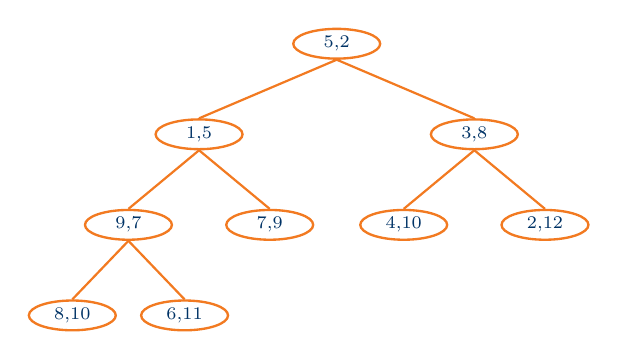
\begin{tikzpicture}[scale=0.92, transform shape,
					grow=down,
					level 1/.style={level distance=1.25cm, sibling distance=3.80cm},
					level 2/.style={level distance=1.25cm, sibling distance=1.95cm},
					level 3/.style={level distance=1.25cm, sibling distance=1.55cm}
					]
					\definecolor{pqorange}{RGB}{242,122,33}
					\tikzset{
						pqnode/.style={
							shape=ellipse,
							draw=pqorange,
							line width=0.85pt,
							fill=white,
							minimum width=12mm,
							minimum height=0mm,
							inner sep=1.2pt,
							font=\scriptsize,
							text=HUSTBlue
						},
						pqedge/.style={draw=pqorange,line width=0.8pt},
						edge from parent/.style={pqedge},
						edge from parent path={(\tikzparentnode.south) -- (\tikzchildnode.north)}
					}
					
					\node[pqnode]{5,2}
					child { node[pqnode]{1,5}
						child { node[pqnode]{9,7}
							child { node[pqnode]{8,10} }
							child { node[pqnode]{6,11} }
						}
						child { node[pqnode]{7,9} }
					}
					child { node[pqnode]{3,8}
						child { node[pqnode]{4,10} }
						child { node[pqnode]{2,12} }
					};
				\end{tikzpicture}
			\end{column}
		\end{columns}
	\end{frame}
	
	%==================== SLIDE: push(v, d[v]) ====================
	\begin{frame}[t]{THUẬT TOÁN DIJKSTRA VÀ CẤU TRÚC PRIORITY QUEUE}
		\small
		\setlength{\leftmargini}{-1.2em}
		
		\begin{columns}[T,onlytextwidth]
			%==================== LEFT: bullet ====================
			\begin{column}{0.45\textwidth}
				\begin{itemize}
					\item Thao tác push($v$, $d[v]$)
					\begin{itemize}
						\item Tạo ra 1 phần tử mới định danh $v$ và khóa $d[v]$
						\item Thêm phần tử mới này vào cuối Min-Heap (cuối mảng)
						\item Lặp lại việc hoán đổi phần tử này với phần tử cha của nó chừng nào khóa của phần tử này nhỏ hơn khóa của cha (thao tác này gọi là UpHeap).
					\end{itemize}
				\end{itemize}
			\end{column}
			
			%==================== RIGHT: heap picture ====================
			\begin{column}{0.50\textwidth}
				\centering
				\vspace{0.9cm}
				
				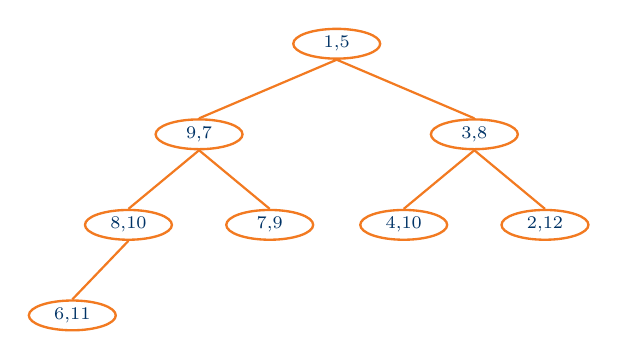
\begin{tikzpicture}[scale=0.92, transform shape,
					grow=down,
					level 1/.style={level distance=1.25cm, sibling distance=3.80cm},
					level 2/.style={level distance=1.25cm, sibling distance=1.95cm},
					level 3/.style={level distance=1.25cm, sibling distance=1.55cm},
					level 4/.style={level distance=1.25cm, sibling distance=1.55cm}
					]
					\definecolor{pqorange}{RGB}{242,122,33}
					\tikzset{
						pqnode/.style={
							shape=ellipse,
							draw=pqorange,
							line width=0.85pt,
							fill=white,
							minimum width=12mm,
							minimum height=0mm,
							inner sep=1.2pt,
							font=\scriptsize,
							text=HUSTBlue
						},
						pqedge/.style={draw=pqorange,line width=0.8pt},
						edge from parent/.style={pqedge},
						edge from parent path={(\tikzparentnode.south) -- (\tikzchildnode.north)}
					}
					
					\node[pqnode]{1,5}
					child { node[pqnode]{9,7}
						child { node[pqnode]{8,10}
							child { node[pqnode]{6,11} }
							child[missing] {} % để 6,11 nằm đúng vị trí con trái
						}
						child { node[pqnode]{7,9} }
					}
					child { node[pqnode]{3,8}
						child { node[pqnode]{4,10} }
						child { node[pqnode]{2,12} }
					};
				\end{tikzpicture}
				
				\vspace{1.25cm}
				{\normalsize Thực hiện thao tác push(5, 6)}
			\end{column}
		\end{columns}
	\end{frame}
	
	%==================== SLIDE: push(5,6) - minh hoạ UpHeap từng bước ====================
	\begin{frame}[t]{THUẬT TOÁN DIJKSTRA VÀ CẤU TRÚC PRIORITY QUEUE}
		\vspace{0.55cm}
		\centering
		
		\definecolor{pqorange}{RGB}{242,122,33}
		
		% style chung
		\tikzset{
			pqnode/.style={
				shape=ellipse,
				draw=pqorange,
				line width=0.85pt,
				fill=white,
				minimum width=12mm,
				minimum height=6.0mm,
				inner sep=1.1pt,
				font=\scriptsize,
				text=HUSTBlue
			},
			pqhot/.style={
				shape=ellipse,
				draw=pqorange,
				line width=0.85pt,
				fill=pqorange,
				minimum width=12mm,
				minimum height=6.0mm,
				inner sep=1.1pt,
				font=\scriptsize,
				text=black
			},
			pqedge/.style={draw=pqorange,line width=0.8pt},
			pqedgehi/.style={draw=pqorange,line width=2.2pt},
			pqmove/.style={draw=pqorange, densely dotted, line width=0.9pt, -{Stealth[length=2.6mm,width=2.6mm]}},
		}
		
		\begin{columns}[T,onlytextwidth]
			%==================== FIG 1 ====================
			\begin{column}{0.31\textwidth}
				\centering
				\begin{adjustbox}{width=\linewidth}
					\begin{tikzpicture}[
						grow=down, transform shape,
						level 1/.style={level distance=1.15cm, sibling distance=3.15cm},
						level 2/.style={level distance=1.15cm, sibling distance=1.90cm},
						level 3/.style={level distance=1.15cm, sibling distance=1.55cm},
						level 4/.style={level distance=1.15cm, sibling distance=1.45cm},
						edge from parent/.style={pqedge},
						edge from parent path={(\tikzparentnode.south) -- (\tikzchildnode.north)}
						]
						\node[pqnode] (r1){1,5}
						child { node[pqnode] (a1){9,7}
							child { node[pqnode] (b1){8,10}
								child { node[pqnode] (c1){6,11} }
								child[edge from parent/.style={pqedgehi}] { node[pqhot] (x1){5,6} }
							}
							child { node[pqnode] (d1){7,9} }
						}
						child { node[pqnode] (e1){3,8}
							child { node[pqnode] (f1){4,10} }
							child { node[pqnode] (g1){2,12} }
						};
					\end{tikzpicture}
				\end{adjustbox}
			\end{column}
			
			%==================== ARROW ====================
			\begin{column}{0.035\textwidth}
				\centering
				\vspace{1.55cm}
				
\begin{tikzpicture}
					\draw[-{Stealth[length=4.2mm,width=4.2mm]}, line width=2.6pt, draw=HUSTBlue]
					(0,0)--(0.95,0);
				\end{tikzpicture}
			\end{column}
			
			%==================== FIG 2 ====================
			\begin{column}{0.31\textwidth}
				\centering
				\begin{adjustbox}{width=\linewidth}
					\begin{tikzpicture}[
						grow=down, transform shape,
						level 1/.style={level distance=1.15cm, sibling distance=3.15cm},
						level 2/.style={level distance=1.15cm, sibling distance=1.90cm},
						level 3/.style={level distance=1.15cm, sibling distance=1.55cm},
						level 4/.style={level distance=1.15cm, sibling distance=1.45cm},
						edge from parent/.style={pqedge},
						edge from parent path={(\tikzparentnode.south) -- (\tikzchildnode.north)}
						]
						% (2) Minh hoạ UpHeap lần 1: cấu trúc CHƯA đổi, chỉ vẽ mũi tên chấm
						\node[pqnode] (r2){1,5}
						child { node[pqnode] (a2){9,7}
							child { node[pqnode] (b2){8,10}
								child { node[pqnode] (c2){6,11} }
								child[edge from parent/.style={pqedgehi}] { node[pqhot] (x2){5,6} }
							}
							child { node[pqnode] (d2){7,9} }
						}
						child { node[pqnode] (e2){3,8}
							child { node[pqnode] (f2){4,10} }
							child { node[pqnode] (g2){2,12} }
						};
						
						% ====== 2 mũi tên 2 hướng (swap) ======
						% 5,6 đi lên vị trí của 8,10 (cung bên trái)
						\draw[pqmove] (x2.north west) to[out=135,in=-70,looseness=1.15] (b2.south west);
						% 8,10 đi xuống vị trí của 5,6 (cung bên phải)
						\draw[pqmove] (b2.south east) to[out=-45,in=70,looseness=1.15] (x2.north east);
					\end{tikzpicture}
				\end{adjustbox}
			\end{column}
			
			%==================== ARROW ====================
			\begin{column}{0.035\textwidth}
				\centering
				\vspace{1.55cm}
				
\begin{tikzpicture}
					\draw[-{Stealth[length=4.2mm,width=4.2mm]}, line width=2.6pt, draw=HUSTBlue]
					(0,0)--(0.95,0);
				\end{tikzpicture}
			\end{column}
			
			%==================== FIG 3 ====================
			\begin{column}{0.31\textwidth}
				\centering
				\begin{adjustbox}{width=\linewidth}
					\begin{tikzpicture}[
						grow=down, transform shape,
						level 1/.style={level distance=1.15cm, sibling distance=3.15cm},
						level 2/.style={level distance=1.15cm, sibling distance=1.90cm},
						level 3/.style={level distance=1.15cm, sibling distance=1.55cm},
						level 4/.style={level distance=1.15cm, sibling distance=1.45cm},
						edge from parent/.style={pqedge},
						edge from parent path={(\tikzparentnode.south) -- (\tikzchildnode.north)}
						]
						\node[pqnode] (r3){1,5}
						child { node[pqnode] (a3){9,7}
							child { node[pqhot] (x3){5,6}
								child { node[pqnode] (c3){6,11} }
								child[edge from parent/.style={pqedgehi}] { node[pqnode] (b3){8,10} }
							}
							child { node[pqnode] (d3){7,9} }
						}
						child { node[pqnode] (e3){3,8}
							child { node[pqnode] (f3){4,10} }
							child { node[pqnode] (g3){2,12} }
						};
						
						% mũi tên cong chấm: tiếp tục UpHeap, xét đổi với 9,7
						\draw[pqmove] (x3.north west) to[out=135,in=-80,looseness=1.15] (a3.south west);
						\draw[pqmove] (a3.south east) to[out=-45,in=80,looseness=1.15] (x3.north east);
					\end{tikzpicture}
				\end{adjustbox}
			\end{column}
		\end{columns}
	\end{frame}
	
	%==================== SLIDE: deleteMin() ====================
	\begin{frame}[t]{THUẬT TOÁN DIJKSTRA VÀ CẤU TRÚC PRIORITY QUEUE}
		\small
		\setlength{\leftmargini}{-1.2em}
		
		\begin{columns}[T,onlytextwidth]
			%==================== LEFT: bullet ====================
			\begin{column}{0.55\textwidth}
				\begin{itemize}
					\item Thao tác deleteMin()
					\begin{itemize}
						\item Hoán đổi phần tử đầu tiên (gốc của Min-Heap) với phần tử cuối cùng của mảng
						\item Thực hiện lặp lại việc hoán đổi phần tử hiện tại (xuất phát từ gốc) với phần tử có khóa nhỏ hơn trong số 2
						phần tử con (nếu có) chừng nào khóa của phần tử hiện tại còn chưa nhỏ hơn hoặc bằng khóa của các phần tử con
						(thao tác này còn được gọi là DownHeap)
						\item Loại bỏ phần tử cuối cùng của mảng đi
					\end{itemize}
				\end{itemize}
			\end{column}
			
			%==================== RIGHT: heap picture ====================
			\begin{column}{0.45\textwidth}
				\centering
				\vspace{0.55cm}
				
				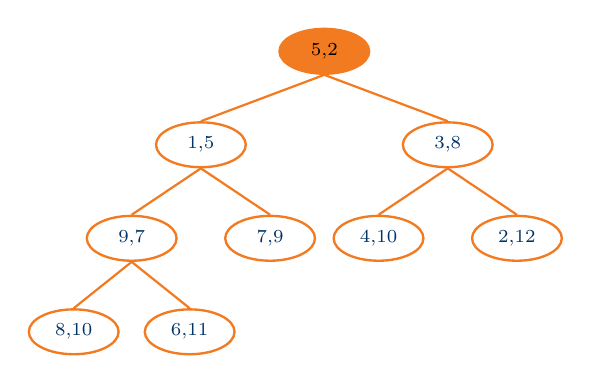
\begin{tikzpicture}[
					scale=0.95, transform shape,
					grow=down,
					level 1/.style={level distance=1.25cm, sibling distance=3.30cm},
					level 2/.style={level distance=1.25cm, sibling distance=1.85cm},
					level 3/.style={level distance=1.25cm, sibling distance=1.55cm}
					]
					\definecolor{pqorange}{RGB}{242,122,33}
					\tikzset{
						pqnode/.style={
							shape=ellipse,
							draw=pqorange,
							line width=0.85pt,
							fill=white,
							minimum width=12mm,
							minimum height=6.0mm,
							inner sep=1.2pt,
							font=\scriptsize,
							text=HUSTBlue
						},
						pqhot/.style={
							shape=ellipse,
							draw=pqorange,
							line width=0.85pt,
							fill=pqorange,
							minimum width=12mm,
							minimum height=6.0mm,
							inner sep=1.2pt,
							font=\scriptsize,
							text=black
						},
						pqedge/.style={draw=pqorange, line width=0.8pt},
						edge from parent/.style={pqedge},
						edge from parent path={(\tikzparentnode.south) -- (\tikzchildnode.north)}
					}
					
					\node[pqhot]{5,2}
					child { node[pqnode]{1,5}
						child { node[pqnode]{9,7}
							child { node[pqnode]{8,10} }
							child { node[pqnode]{6,11} }
						}
						child { node[pqnode]{7,9} }
					}
					child { node[pqnode]{3,8}
						child { node[pqnode]{4,10} }
						child { node[pqnode]{2,12} }
					};
				\end{tikzpicture}
			\end{column}
		\end{columns}
	\end{frame}
	
	
	\begin{frame}[t]{THUẬT TOÁN DIJKSTRA VÀ CẤU TRÚC PRIORITY QUEUE}
		\vspace{-0.3cm}
		\centering
		
		\definecolor{pqorange}{RGB}{242,122,33}
		
		\tikzset{
			pqnode/.style={
				shape=ellipse, draw=pqorange, line width=0.85pt, fill=white,
				minimum width=12mm, minimum height=6.0mm, inner sep=1.1pt,
				font=\scriptsize, text=HUSTBlue
			},
			pqhot/.style={
				shape=ellipse, draw=pqorange, line width=0.85pt, fill=pqorange,
				minimum width=12mm, minimum height=6.0mm, inner sep=1.1pt,
				font=\scriptsize, text=black
			},
			pqedge/.style={draw=pqorange,line width=0.8pt},
			pqmove/.style={draw=pqorange, densely dotted, line width=0.9pt, -{Stealth[length=2.6mm,width=2.6mm]}},
		}
		
		%==================== TOP ROW ====================
		\begin{columns}[T,onlytextwidth]
			%----- TOP-LEFT (A)
			\hspace*{-0.6cm}
			\begin{column}{0.31\textwidth}
				\centering
				\begin{adjustbox}{width=\linewidth}
					\begin{tikzpicture}[
						grow=down, transform shape,
						level 1/.style={level distance=1.05cm, sibling distance=3.05cm},
						level 2/.style={level distance=1.05cm, sibling distance=1.90cm},
						level 3/.style={level distance=1.05cm, sibling distance=1.55cm},
						edge from parent/.style={pqedge},
						edge from parent path={(\tikzparentnode.south) -- (\tikzchildnode.north)}
						]
						\node[pqhot] (A_r){5,2}
						child{ node[pqnode] (A_l){1,5}
							child{ node[pqnode] (A_ll){9,7}
								child{ node[pqnode] {8,10} }
								child{ node[pqnode] (A_last){6,11} }
							}
							child{ node[pqnode] {7,9} }
						}
						child{ node[pqnode] (A_rt){3,8}
							child{ node[pqnode] {4,10} }
							child{ node[pqnode] {2,12} }
						};
					\end{tikzpicture}
				\end{adjustbox}
			\end{column}
			
			%----- ARROW ->
			\hspace*{0.5cm}
			\begin{column}{0.035\textwidth}
				\centering
				\vspace{1.30cm}
				
\begin{tikzpicture}
					\draw[-{Stealth[length=4.2mm,width=4.2mm]}, line width=2.6pt, draw=HUSTBlue]
					(0,0)--(0.95,0);
				\end{tikzpicture}
			\end{column}
			
			%----- TOP-MIDDLE (B) : swap root <-> last (2 arrows)
			\begin{column}{0.31\textwidth}
				\centering
				\begin{adjustbox}{width=\linewidth}
					\begin{tikzpicture}[
						grow=down, transform shape,
						level 1/.style={level distance=1.05cm, sibling distance=3.05cm},
						level 2/.style={level distance=1.05cm, sibling distance=1.90cm},
						level 3/.style={level distance=1.05cm, sibling distance=1.55cm},
						edge from parent/.style={pqedge},
						edge from parent path={(\tikzparentnode.south) -- (\tikzchildnode.north)}
						]
						\node[pqhot] (B_r){5,2}
						child{ node[pqnode] (B_l){1,5}
							child{ node[pqnode] (B_ll){9,7}
								child{ node[pqnode] {8,10} }
								child{ node[pqnode] (B_last){6,11} }
							}
							child{ node[pqnode] {7,9} }
						}
						child{ node[pqnode] {3,8}
							child{ node[pqnode] {4,10} }
							child{ node[pqnode] {2,12} }
						};
						
						% 2 mũi tên 2 hướng (swap 5,2 <-> 6,11)
						\draw[pqmove] (B_r.north west) to[out=160,in=110,looseness=1.18] (B_last.south west);
						\draw[pqmove] (B_last.south east) to[out=-70,in=-20,looseness=1.18] (B_r.north east);
					\end{tikzpicture}
				\end{adjustbox}
			\end{column}
			
			%----- ARROW ->
			\begin{column}{0.035\textwidth}
				\centering
				\vspace{1.30cm}
				
\begin{tikzpicture}
					\draw[-{Stealth[length=4.2mm,width=4.2mm]}, line width=2.6pt, draw=HUSTBlue]
					(0,0)--(0.95,0);
				\end{tikzpicture}
			\end{column}
			
			%----- TOP-RIGHT (C) : after swap, downheap step (6,11 <-> 1,5) (2 arrows)
			
			\begin{column}{0.31\textwidth}
				\centering
				\hspace*{0.5cm}
				\begin{adjustbox}{width=\linewidth}
					\begin{tikzpicture}[
						grow=down, transform shape,
						level 1/.style={level distance=1.05cm, sibling distance=3.05cm},
						level 2/.style={level distance=1.05cm, sibling distance=1.90cm},
						level 3/.style={level distance=1.05cm, sibling distance=1.55cm},
						edge from parent/.style={pqedge},
						edge from parent path={(\tikzparentnode.south) -- (\tikzchildnode.north)}
						]
						\node[pqnode] (C_r){6,11}
						child{ node[pqnode] (C_l){1,5}
							child{ node[pqnode] (C_ll){9,7}
								child{ node[pqnode] {8,10} }
								child{ node[pqhot] {5,2} }
							}
							child{ node[pqnode] {7,9} }
						}
						child{ node[pqnode] {3,8}
							child{ node[pqnode] {4,10} }
							child{ node[pqnode] {2,12} }
						};
						
						% 2 mũi tên 2 hướng (swap 6,11 <-> 1,5)
						\draw[pqmove] (C_r.north west) to[out=165,in=110,looseness=1.10] (C_l.south west);
						\draw[pqmove] (C_l.south east) to[out=-70,in=-15,looseness=1.10] (C_r.north east);
					\end{tikzpicture}
				\end{adjustbox}
			\end{column}
		\end{columns}
		
		%----- DOWN ARROW under TOP-RIGHT
		\vspace{-0.75cm}
		\begin{columns}[T,onlytextwidth]
			\begin{column}{0.31\textwidth}\end{column}
			\begin{column}{0.035\textwidth}\end{column}
			\begin{column}{0.31\textwidth}\end{column}
			\begin{column}{0.035\textwidth}\end{column}
			\begin{column}{0.31\textwidth}
				\centering
				
\begin{tikzpicture}
					\draw[-{Stealth[length=4.2mm,width=4.2mm]}, line width=2.6pt, draw=HUSTBlue]
					(0,0.55)--(0,-0.55);
				\end{tikzpicture}
			\end{column}
		\end{columns}
		
		\vspace{0.55cm}
		
		%==================== BOTTOM ROW (left <- middle <- right) ====================
		\begin{columns}[T,onlytextwidth]
			%----- BOTTOM-LEFT (F) : final (no dotted)
			\hspace*{-0.6cm}
			\begin{column}{0.31\textwidth}
				\centering
				\begin{adjustbox}{width=\linewidth}
					\begin{tikzpicture}[
						grow=down, transform shape,
						level 1/.style={level distance=1.05cm, sibling distance=3.05cm},
						level 2/.style={level distance=1.05cm, sibling distance=1.90cm},
						level 3/.style={level distance=1.05cm, sibling distance=1.55cm},
						edge from parent/.style={pqedge},
						edge from parent path={(\tikzparentnode.south) -- (\tikzchildnode.north)}
						]
						\node[pqnode] {1,5}
						child{ node[pqnode] {9,7}
							child{ node[pqnode] {8,10}
								child{ node[pqnode] {6,11} }
								child{ node[pqhot] {5,2} }
							}
							child{ node[pqnode] {7,9} }
						}
						child{ node[pqnode] {3,8}
							child{ node[pqnode] {4,10} }
							child{ node[pqnode] {2,12} }
						};
					\end{tikzpicture}
				\end{adjustbox}
			\end{column}
			
			%----- ARROW <-
			\hspace*{-0.2cm}
			\begin{column}{0.035\textwidth}
				\centering
				\vspace{1.30cm}
				
\begin{tikzpicture}
					\draw[-{Stealth[length=4.2mm,width=4.2mm]}, line width=2.6pt, draw=HUSTBlue]
					(0.95,0)--(0,0);
				\end{tikzpicture}
			\end{column}
			
			%----- BOTTOM-MIDDLE (E) : swap 6,11 <-> 8,10 (2 arrows)
			\hspace*{-0.1cm}
			\begin{column}{0.31\textwidth}
				\centering
				\begin{adjustbox}{width=\linewidth}
					\begin{tikzpicture}[
						grow=down, transform shape,
						level 1/.style={level distance=1.05cm, sibling distance=3.05cm},
						level 2/.style={level distance=1.05cm, sibling distance=1.90cm},
						level 3/.style={level distance=1.05cm, sibling distance=1.55cm},
						edge from parent/.style={pqedge},
						edge from parent path={(\tikzparentnode.south) -- (\tikzchildnode.north)}
						]
						\node[pqnode] {1,5}
						child{ node[pqnode] {9,7}
							child{ node[pqnode] (E_x){6,11}
								child{ node[pqnode] (E_y){8,10} }
								child{ node[pqhot] {5,2} }
							}
							child{ node[pqnode] {7,9} }
						}
						child{ node[pqnode] {3,8}
							child{ node[pqnode] {4,10} }
							child{ node[pqnode] {2,12} }
						};
						
						% 2 mũi tên 2 hướng (swap 6,11 <-> 8,10)
						\draw[pqmove] (E_x.north west) to[out=170,in=110,looseness=1.08] (E_y.south west);
						\draw[pqmove] (E_y.south east) to[out=-70,in=-10,looseness=1.08] (E_x.north east);
					\end{tikzpicture}
				\end{adjustbox}
			\end{column}
			
			%----- ARROW <-
			\begin{column}{0.035\textwidth}
				\centering
				\vspace{1.30cm}
				
\begin{tikzpicture}
					\draw[-{Stealth[length=4.2mm,width=4.2mm]}, line width=2.6pt, draw=HUSTBlue]
					(0.95,0)--(0,0);
				\end{tikzpicture}
			\end{column}
			
			%----- BOTTOM-RIGHT (D) : swap 6,11 <-> 9,7 (2 arrows)
			
			\begin{column}{0.31\textwidth}
				\centering
				\begin{adjustbox}{width=\linewidth}
					\begin{tikzpicture}[
						grow=down, transform shape,
						level 1/.style={level distance=1.05cm, sibling distance=3.05cm},
						level 2/.style={level distance=1.05cm, sibling distance=1.90cm},
						level 3/.style={level distance=1.05cm, sibling distance=1.55cm},
						edge from parent/.style={pqedge},
						edge from parent path={(\tikzparentnode.south) -- (\tikzchildnode.north)}
						]
						\node[pqnode] {1,5}
						child{ node[pqnode] (D_x){6,11}
							child{ node[pqnode] (D_y){9,7}
								child{ node[pqnode] {8,10} }
								child{ node[pqhot] {5,2} }
							}
							child{ node[pqnode] {7,9} }
						}
						child{ node[pqnode] {3,8}
							child{ node[pqnode] {4,10} }
							child{ node[pqnode] {2,12} }
						};
						
						% 2 mũi tên 2 hướng (swap 6,11 <-> 9,7)
						\draw[pqmove] (D_x.north west) to[out=165,in=110,looseness=1.10] (D_y.south west);
						\draw[pqmove] (D_y.south east) to[out=-70,in=-15,looseness=1.10] (D_x.north east);
					\end{tikzpicture}
				\end{adjustbox}
			\end{column}
		\end{columns}
		
	\end{frame}
	
	%==================== SLIDE: Dijkstra dùng Priority Queue ====================
	\begin{frame}[t,fragile]{THUẬT TOÁN DIJKSTRA VÀ CẤU TRÚC PRIORITY QUEUE}
		\vspace*{-0.4cm}
		\setlength{\leftmargini}{-1.2em}
		
		\begin{columns}[T,onlytextwidth]
			%==================== LEFT: bullet ====================
			\begin{column}{0.45\textwidth}
				\begin{itemize}
					\item Thuật toán Dijkstra sử dụng hàng đợi ưu tiên
					\begin{itemize}
						\item Khởi tạo hàng đợi ưu tiên \texttt{pq} chứa các\\
						đỉnh đã tìm được đường đi cận trên đồng\\
						thời chưa tìm được đường đi ngắn nhất
						
						\item Mỗi bước lặp sẽ dùng thao tác \texttt{deleteMin()}\\
						để lấy ra đỉnh $u$ từ \texttt{pq} có $d[u]$ nhỏ nhất và\\
						cập nhật lại $d[v]$ với mỗi đỉnh $v$ kề với $u$\\
						nếu $d[v] > d[u] + c(u,v)$ sau đó \texttt{push}$(v,d[v])$\\
						vào \texttt{pq}
					\end{itemize}
				\end{itemize}
			\end{column}
			
			%==================== RIGHT: pseudocode box ====================
			\begin{column}{0.50\textwidth}
				\vspace{-0.2em}
				\begin{tcolorbox}[
					colback=white,
					colframe=HUSTBlue,
					boxrule=0.6pt,
					arc=0pt,
					boxsep=0pt,
					left=-40pt,right=8pt,top=8pt,bottom=8pt,
					height=0.78\textheight,
					valign=top
					]
					\begin{minted}[fontsize=\footnotesize,linenos=false]{text}
						Dijkstra(G = (V, A), s, t){
							for v in V do d[v] = +∞;
							
							pq = initPQ(); pq.push(s, 0);
							
							while(pq not empty){
								u = pq.deleteMin();
								for e in A[u] do {
									v = e.id; w = e.w;
									
									if d[v] > d[u] + w then
									pq.push(v, d[u] + w);
								}
							}
							
							return d[t];
						}
					\end{minted}
				\end{tcolorbox}
			\end{column}
		\end{columns}
	\end{frame}
	
	%==================== SLIDE 28: Minh hoạ vào/ra (Dijkstra) ====================
	\begin{frame}[t]{THUẬT TOÁN DIJKSTRA VÀ CẤU TRÚC PRIORITY QUEUE}
		\small
		\setlength{\leftmargini}{-1.2em}
		
		\begin{columns}[T,onlytextwidth]
			%==================== LEFT: bullet ====================
			\begin{column}{0.62\textwidth}
				\begin{itemize}
					\item Minh hoạ với ngôn ngữ C
					
					\item Dữ liệu
					\begin{itemize}
						\item Dòng 1: ghi 2 số nguyên dương $n$ và $m$ tương ứng là số đỉnh và\\
						số cung của $G$ $(1 \le n, m \le 10^5)$
						
						\item Dòng $i$ $(i = 1,2,\ldots,m)$: ghi 3 số nguyên dương $u$, $v$ và $c$ trong đó\\
						$c$ là trọng số cung $(u,v)$
						
						\item Dòng cuối cùng chứa 2 số nguyên dương là đỉnh $s$ (đỉnh đầu) và $t$\\
						(đỉnh cuối)
					\end{itemize}
					
					\item Kết quả
					\begin{itemize}
						\item Ghi ra trọng số của đường đi ngắn nhất từ $s$ đến $t$
					\end{itemize}
				\end{itemize}
			\end{column}
			
			%==================== RIGHT: I/O table ====================
			\begin{column}{0.30\textwidth}
				\centering
				\vspace{0.75cm}
				
				\renewcommand{\arraystretch}{1.15}
				\setlength{\tabcolsep}{8pt}
				
				\begin{tabular}{|p{0.55\linewidth}|p{0.33\linewidth}|}
					\hline
					\textbf{stdin} & \textbf{stdout} \\
					\hline
					\begin{minipage}[t]{\linewidth}\raggedright\footnotesize
						5 7\\
						2 5 87\\
						1 2 97\\
						4 5 78\\
						3 1 72\\
						1 4 19\\
						2 3 63\\
						5 1 18\\
						1 5
					\end{minipage}
					&
					\begin{minipage}[t]{\linewidth}\raggedright\footnotesize
						97
					\end{minipage}
					\\
					\hline
				\end{tabular}
			\end{column}
		\end{columns}
	\end{frame}
	
	
	%==================== SLIDE 29: Code (khai báo) ====================
	\begin{frame}[t,fragile]{THUẬT TOÁN DIJKSTRA VÀ CẤU TRÚC PRIORITY QUEUE}
		\vspace{-0.45cm}
		\setlength{\leftmargini}{-1.2em}
		
		\begin{columns}[T,onlytextwidth]
			%==================== LEFT CODE BOX ====================
			\hspace*{-0.9cm}
			\begin{column}{0.33\textwidth}
				\begin{tcolorbox}[
					colback=white,
					colframe=HUSTBlue,
					boxrule=0.6pt,
					arc=0pt,
					left=-40pt,right=8pt,top=8pt,bottom=8pt,
					]
					\begin{minted}[fontsize=\scriptsize,linenos=false]{c}
						#include <stdio.h>
						#include <stdlib.h>
						#define N 100001
						#define INF 1000000
						
						typedef struct Arc{
							int id;
							int w;
							struct Arc* next;
						}Arc;
					\end{minted}
				\end{tcolorbox}
			\end{column}
			
			%==================== RIGHT CODE BOX ====================
			\hspace*{0.2cm}
			\begin{column}{0.77\textwidth}
				\begin{tcolorbox}[
					colback=white,
					colframe=HUSTBlue,
					boxrule=0.6pt,
					arc=0pt,
					left=-50pt,right=8pt,top=8pt,bottom=8pt,
					]
					\begin{minted}[fontsize=\scriptsize,linenos=false]{c}
						int n,m; // number of nodes and arcs of the given graph
						int s,t; // source and destination nodes
						Arc* A[N];//A[v] is the pointer to the first item of the adjacent arcs
						// of node v
						
						// priority queue data structure (implemented using BINARY HEAP)
						int d[N];// d[v] is the upper bound of the length of the shortest path
						// from s to v (key)
						int node[N]; // node[i] the i-th element in the HEAP
						int idx[N];  // idx[v] is the index of v in the HEAP (idx[node[i]] = i)
						int szH;     // size of the HEAP
					\end{minted}
				\end{tcolorbox}
			\end{column}
		\end{columns}
	\end{frame}
	
	%==================== SLIDE 30: Heap utils (swap, upHeap, inHeap, downHeap) ====================
	\begin{frame}[t,fragile]{THUẬT TOÁN DIJKSTRA VÀ CẤU TRÚC PRIORITY QUEUE}
		\vspace{-0.45cm}
		\setlength{\leftmargini}{-1.2em}
		
		\begin{columns}[T,onlytextwidth]
			%==================== LEFT BOX ====================
			\begin{column}{0.49\textwidth}
				\begin{tcolorbox}[
					colback=white,
					colframe=HUSTBlue,
					boxrule=0.6pt,
					arc=0pt,
					left=-50pt,right=8pt,top=8pt,bottom=8pt,
					]
					\begin{minted}[fontsize=\scriptsize,linenos=false]{c}
						void swap(int i, int j){
							int tmp = node[i]; node[i] = node[j];
							node[j] = tmp;
							idx[node[i]] = i; idx[node[j]] = j;
						}
						
						void upHeap(int i){
							if(i == 0) return;
							while(i > 0){
								int pi = (i-1)/2;
								if(d[node[i]] < d[node[pi]]) swap(i,pi);
								else break;
								i = pi;
							}
						}
					\end{minted}
				\end{tcolorbox}
			\end{column}
			
			%==================== RIGHT BOX ====================
			\begin{column}{0.49\textwidth}
				\begin{tcolorbox}[
					colback=white,
					colframe=HUSTBlue,
					boxrule=0.6pt,
					arc=0pt,
					left=-52pt,right=8pt,top=8pt,bottom=8pt,
					]
					\begin{minted}[fontsize=\scriptsize,linenos=false]{c}
						int inHeap(int v){
							return idx[v] >= 0;
						}
						
						void downHeap(int i){
							int L = 2*i+1; int R = 2*i+2;
							
							int maxIdx = i;
							if(L < szH && d[node[L]] < d[node[maxIdx]])
							maxIdx = L;
							
							if(R < szH && d[node[R]] < d[node[maxIdx]])
							maxIdx = R;
							
							if(maxIdx != i){
								swap(i,maxIdx); downHeap(maxIdx);
							}
						}
					\end{minted}
				\end{tcolorbox}
			\end{column}
		\end{columns}
	\end{frame}
	
	
	%==================== SLIDE 31: updateKey / pushPQ / pqEmpty / deleteMin ====================
	\begin{frame}[t,fragile]{THUẬT TOÁN DIJKSTRA VÀ CẤU TRÚC PRIORITY QUEUE}
		\vspace{-0.45cm}
		\setlength{\leftmargini}{-1.2em}
		
		\begin{columns}[T,onlytextwidth]
			%==================== LEFT BOX ====================
			\begin{column}{0.49\textwidth}
				\begin{tcolorbox}[
					colback=white,
					colframe=HUSTBlue,
					boxrule=0.6pt,
					arc=0pt,
					left=-50pt,right=8pt,top=8pt,bottom=8pt,
					]
					\begin{minted}[fontsize=\scriptsize,linenos=false]{c}
						void updateKey(int v, int k){
							if(d[v] > k){ d[v] = k; upHeap(idx[v]); }
							else{ d[v] = k; downHeap(idx[v]); }
						}
						
						void pushPQ(int v, int k){
							if(!inHeap(v)){
								d[v] = k;      node[szH] = v;
								idx[node[szH]] = szH;  upHeap(szH);
								szH++;
							}else updateKey(v,k);
						}
					\end{minted}
				\end{tcolorbox}
			\end{column}
			
			%==================== RIGHT BOX ====================
			\begin{column}{0.49\textwidth}
				\begin{tcolorbox}[
					colback=white,
					colframe=HUSTBlue,
					boxrule=0.6pt,
					arc=0pt,
					left=-40pt,right=8pt,top=8pt,bottom=8pt,
					]
					\begin{minted}[fontsize=\scriptsize,linenos=false]{c}
						int pqEmpty(){
							return szH <= 0;
						}
						
						int deleteMin(){
							int sel_node = node[0];
							swap(0,szH-1); szH--; downHeap(0);
							return sel_node;
						}
					\end{minted}
				\end{tcolorbox}
			\end{column}
		\end{columns}
	\end{frame}
	
	%==================== SLIDE 32: makeArc / addArc / input ====================
	\begin{frame}[t,fragile]{THUẬT TOÁN DIJKSTRA VÀ CẤU TRÚC PRIORITY QUEUE}
		\vspace{-0.45cm}
		\setlength{\leftmargini}{-1.2em}
		
		\begin{columns}[T,onlytextwidth]
			%==================== LEFT BOX ====================
			\begin{column}{0.49\textwidth}
				\begin{tcolorbox}[
					colback=white,
					colframe=HUSTBlue,
					boxrule=0.6pt,
					arc=0pt,
					left=-40pt,right=8pt,top=8pt,bottom=8pt,
					]
					\begin{minted}[fontsize=\scriptsize,linenos=false]{c}
						Arc* makeArc(int id, int w){
							Arc* a = (Arc*)malloc(sizeof(Arc));
							a->id = id; a->w = w; a->next = NULL; 
							return a;
						}
						
						void addArc(int u, int v, int w){
							Arc* a = makeArc(v,w);
							a->next = A[u]; A[u] = a;
						}
					\end{minted}
				\end{tcolorbox}
			\end{column}
			
			%==================== RIGHT BOX ====================
			\begin{column}{0.49\textwidth}
				\begin{tcolorbox}[
					colback=white,
					colframe=HUSTBlue,
					boxrule=0.6pt,
					arc=0pt,
					left=-40pt,right=8pt,top=8pt,bottom=8pt,
					]
					\begin{minted}[fontsize=\scriptsize,linenos=false]{c}
						void input(){
							scanf("%d%d",&n,&m);
							for(int v = 1; v <= n; v++) A[v] = NULL;
							for(int k = 1; k <= m; k++){
								int u,v,w;
								scanf("%d%d%d",&u,&v,&w);
								addArc(u,v,w);
							}
							scanf("%d%d",&s,&t);
						}
					\end{minted}
				\end{tcolorbox}
			\end{column}
		\end{columns}
	\end{frame}
	
	
	%==================== SLIDE 33: initPQ / main / solve ====================
	\begin{frame}[t,fragile]{THUẬT TOÁN DIJKSTRA VÀ CẤU TRÚC PRIORITY QUEUE}
		\vspace{-0.45cm}
		\setlength{\leftmargini}{-1.2em}
		
		\begin{columns}[T,onlytextwidth]
			%==================== LEFT COLUMN (2 boxes stacked) ====================
			\begin{column}{0.36\textwidth}
				
				%----- initPQ box (top)
				\begin{tcolorbox}[
					colback=white,
					colframe=HUSTBlue,
					boxrule=0.6pt,
					arc=0pt,
					left=-40pt,right=8pt,top=8pt,bottom=8pt,
					]
					\begin{minted}[fontsize=\scriptsize,linenos=false]{c}
						void initPQ(){
							szH = 0;
							for(int v = 1; v <= n; v++)
							idx[v] = -1;
						}
					\end{minted}
				\end{tcolorbox}
				
				\vspace{0.35cm}
				
				%----- main box (bottom)
				\begin{tcolorbox}[
					colback=white,
					colframe=HUSTBlue,
					boxrule=0.6pt,
					arc=0pt,
					left=-40pt,right=8pt,top=8pt,bottom=8pt,
					]
					\begin{minted}[fontsize=\scriptsize,linenos=false]{c}
						int main(){
							input();
							solve();
							return 0;
						}
					\end{minted}
				\end{tcolorbox}
			\end{column}
			
			%==================== RIGHT: solve box ====================
			\hspace*{0.3cm}
			\begin{column}{0.64\textwidth}
				\begin{tcolorbox}[
					colback=white,
					colframe=HUSTBlue,
					boxrule=0.6pt,
					arc=0pt,
					left=-40pt,right=8pt,top=8pt,bottom=8pt,
					]
					\begin{minted}[fontsize=\scriptsize,linenos=false]{c}
						void solve(){
							for(int v = 1; v <= n; v++) d[v] = INF;
							initPQ(); pushPQ(s,0);
							while(!pqEmpty()){
								int u = deleteMin();
								for(Arc* a = A[u]; a != NULL; a = a->next){
									int v = a->id; int w = a->w;
									if(d[v] > d[u] + w) pushPQ(v,d[u]+w);
								}
							}
							int rs = d[t]; if(d[t]==INF) rs = -1;
							printf("%d",rs);
						}
					\end{minted}
				\end{tcolorbox}
			\end{column}
		\end{columns}
	\end{frame}
	
	
	
	
	
	
	
	
	
	
	
	
	






	
	


{\HUSTUseBackground{theme_hust_oneside.pdf}
	\begin{frame}
		\ifdefstring{\insertaspectratio}{169}{
			\placecontent{0.355\paperwidth}{0.410\paperheight}{0.640\paperwidth}{
				\color{HUSTRed}\bfseries\fontsize{28pt}{36pt}\selectfont\centering
				THANK YOU!
			}
		}{}
		\ifdefstring{\insertaspectratio}{43}{
			\placecontent{0.355\paperwidth}{0.440\paperheight}{0.640\paperwidth}{
				\color{HUSTRed}\bfseries\fontsize{28pt}{36pt}\selectfont\centering
				THANK YOU!
			}
		}{}
	\end{frame}
}



	


	



\end{document}